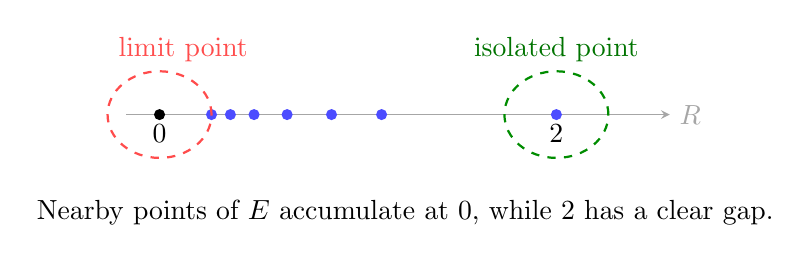
\begin{tikzpicture}[x=1.2cm,y=1cm,>=stealth]
  \draw[->,gray!70] (-0.35,0) -- (5.4,0) node[right] {\(\mathbb{R}\)};
  \foreach \x in {0.55,0.75,1.0,1.35,1.82,2.35}
  {
    \fill[blue!70] (\x,0) circle (2pt);
  }
  \fill[black] (0,0) circle (2pt);
  \node[below] at (0,0) {\(0\)};
  \draw[red!70,thick,dashed] (0,0) circle (0.55);
  \node[red!70,above] at (0.25,0.55) {limit point};

  \fill[blue!70] (4.2,0) circle (2pt);
  \node[below] at (4.2,0) {\(2\)};
  \draw[green!55!black,thick,dashed] (4.2,0) circle (0.55);
  \node[green!45!black,above] at (4.2,0.55) {isolated point};

  \node[align=center] at (2.6,-1.25)
    {Nearby points of \(E\) accumulate at \(0\), while \(2\) has a clear gap.};
\end{tikzpicture}
